\documentclass{article}

\usepackage[final]{nips_2018}

\usepackage[T1]{fontenc}    % use 8-bit T1 fonts

% Useful packages
\usepackage{amsmath, amssymb, amsfonts, bm}
\usepackage{amsthm}
\usepackage{booktabs}       % professional-quality tables
\usepackage{mathtools}
\usepackage{nicefrac}       % compact symbols for 1/2, etc.
\usepackage[usenames, dvipsnames]{color}
\usepackage{multirow}
\usepackage{hyperref}

\usepackage{floatrow}
\floatsetup[table]{capposition=top}

\usepackage{wrapfig}
\usepackage{multicol}

% For gap between cmidrules.
\usepackage{array}
\newcolumntype{C}{@{\extracolsep{0.1cm}}c@{\extracolsep{0pt}}}%

\setlength{\columnsep}{1cm}
\setlength{\columnseprule}{0.5pt}
\def\columnseprulecolor{\color{Plum}}

% Simple macros.
\def\sec#1{Sec.~\ref{#1}}
\def\Sec#1{Sec.~\ref{#1}}
\def\fig#1{Fig.~\ref{#1}}
\def\Fig#1{Fig.~\ref{#1}}
\def\tableref#1{Table~\ref{#1}}

\newcommand{\tk}[1]{\textcolor{red}{TK: #1}}
\newcommand{\tkf}[1]{\footnote{\tk{#1}}}
\newcommand{\ao}[1]{\textcolor{green}{AO: #1}}
\newcommand{\tsj}[1]{\textcolor{magenta}{TSJ: #1}}
\newcommand{\vm}[1]{\textcolor{blue}{Vincent M: #1}}
\newcommand{\vmf}[1]{\footnote{\vm{#1}}}


\newcommand{\cw}{\mathbf{cw}}
\newcommand{\cc}{\mathbf{c}}
\newcommand{\kb}{\mathbf{k}}
\newcommand{\mem}{\mathbf{m}}
\newcommand{\rr}{\mathbf{r}}

\title{On transfer learning using a MAC model variant:\\ supplementary material}

% The \author macro works with any number of authors. There are two
% commands used to separate the names and addresses of multiple
% authors: \And and \AND.
%
% Using \And between authors leaves it to LaTeX to determine where to
% break the lines. Using \AND forces a line break at that point. So,
% if LaTeX puts 3 of 4 authors names on the first line, and the last
% on the second line, try using \AND instead of \And before the third
% author name.

\author{
	\textbf{\null\hfill Vincent Marois \hfill T.S. Jayram \hfill Vincent Albouy  \hfill\null}\\
	\textbf{\null\hfill Tomasz Kornuta \hfill Younes Bouhadjar \hfill Ahmet S. Ozcan \hfill\null}\\
	IBM Research AI, Almaden Research Center, San Jose, USA\\
	\texttt{\{vmarois,jayram,tkornut,byounes,asozcan\}@us.ibm.com}\\
	\texttt{\{vincent.albouy\}@ibm.com}\\
}

\begin{document}
% \nipsfinalcopy is no longer used

\maketitle

% Little cheating to make our names fit:]
\vskip -0.5cm
\begin{abstract}
We introduce a variant of the MAC model (Hudson and Manning, ICLR 2018) with a simplified set of equations that achieves comparable accuracy, while training faster. We evaluate both models on CLEVR and CoGenT, and show that, transfer learning with fine-tuning results in a 15 point increase in accuracy, matching the state of the art. Finally, in contrast, we demonstrate that improper fine-tuning can actually reduce a model's accuracy as well.
\end{abstract}

\appendix

\section{Description of datasets}

Most of the VQA datasets have strong biases. This allow models to learn strategies without reasoning about the visual input~\cite{Santoro2017ASN}.
The CLEVR dataset~\cite{johnson2017clevr} was developed to address those issues and come back to the core challenge of visual QA which is testing reasoning abilities.
CLEVR contains images of 3D-rendered objects; each image comes with a number of highly compositional questions that fall into different categories.
Those categories fall into 5 classes of tasks: Exist, Count, Compare Integer, Query Attribute and Compare Attribute. 
The CLEVR dataset consists of:
\begin{itemize}
\item 	A training set of 70k images and 700k questions,
\item	A validation set of 15k images and 150k questions,
\item	A test  set of 15k images and 150k questions about objects,
\item	Answers, scene graphs and functional programs for all train and val images and questions.
\end{itemize}
Each object present in the scene, aside of position, is characterized by a set of four attributes:
\begin{itemize}
\item 2 sizes: large, small,
\item 3 shapes: square, cylinder, sphere,
\item 2 material types: rubber, metal,
\item 8 color types: gray, blue, brown, yellow, red, green, purple, cyan,
\end{itemize}
resulting in 96 unique combinations.

Along with CLEVR, the authors~\cite{johnson2017clevr} introduced  CLEVR-CoGenT (Compositional Generalization Test, CoGenT in short), with a goal of evaluating how well the models can generalize, learn relations and compositional concepts.
This dataset is generated in the same way as CLEVR with two additional conditions.
As shown in \tableref{tab:cogent_conditions}, in Condition A all cubes are gray, blue, brown, or yellow, whereas all cylinders are red, green, purple, or cyan; in Condition B cubes and cylinders swap color palettes.
For both conditions spheres can be any colors.


The CoGenT dataset contains:
\begin{itemize}
\item	Training set of 70,000 images and 699,960 questions in Condition A,
\item	Validation set of 15,000 images and 149,991 questions in Condition A,
\item	Test set of 15,000 images and 149,980 questions in Condition A (without answers),
\item	Validation set of 15,000 images and 150,000 questions in Condition B,
\item	Test set of 15,000 images and 149,992 questions in Condition B (without answers),
\item	Answers, scene graphs and functional programs for all training and validation images and questions.
\end{itemize}

\begin{table}[h!]
	\centering
	\begin{tabular}{cccc}
		\toprule
		Dataset        & Cubes              & Cylinders &  Spheres         \\
		\midrule
		CLEVR   &  any color &  any color        &    any color    \\
		%\midrule
		CLEVR CoGenT A & gray / blue / brown / yellow  & red / green / purple / cyan       &    any color  \\
		CLEVR CoGenT B  & red / green / purple / cyan &   gray / blue / brown / yellow       &      any color  \\
		\bottomrule
	\end{tabular}
	\caption{Colors/shapes combinations present in CLEVR, CoGenT-A and CoGenT-B datasets}
	\label{tab:cogent_conditions}
\end{table}

 
 \newpage
\section{Full MAC and S-MAC comparison}

In \tableref{tab:results_full} we present the full comparison between MAC and S-MAC models.


\begin{table}[!h]
	\caption{CLEVR \& CoGenT accuracies for the MAC \& S-MAC models}
	\centering
	\begin{tabular}{ccccCcCc}
		\toprule
		\multirow{2}{*}{Model} & \multicolumn{3}{c}{Training} &  \multicolumn{2}{c}{Fine-tuning} &  \multicolumn{2}{c}{Test} \\
		\cmidrule{2-4} \cmidrule{5-6} \cmidrule{7-8} 
		& Dataset                & Time [h:m] & Acc [\%]          & Dataset & Acc [\%]  & Dataset & Acc [\%] \\
		\midrule
		\multirow{15}{*}{MAC} & \multirow{10}{*}{CLEVR}  & \multirow{10}{*}{30:52}  & \multirow{10}{*}{96.70} & \multirow{4}{*}{--}   & \multirow{4}{*}{--}  & CLEVR    & 96.17          \\
		\cmidrule{7-8} 
		&                        &  &               &     &                                & CoGenT-A    &  96.22   \\
		\cmidrule{7-8} 
		&                        &   &              &     &                               & CoGenT-B   & 96.27  \\
		
		\cmidrule{5-6} \cmidrule{7-8} 
		&                             &                                         &    &   \multirow{2}{*}{CoGenT-A}         &       \multirow{2}{*}{98.06}          & CoGenT-A &  94.60	         \\
		\cmidrule{7-8} 
		&                             &                                         &       &         &                & CoGenT-B &    93.28       \\
		\cmidrule{5-6} \cmidrule{7-8} 
		&                             &                                         &    &   \multirow{2}{*}{CoGenT-B}         &       \multirow{2}{*}{98.16}          & CoGenT-A &  93.02         \\
		\cmidrule{7-8} 
		&                             &                                         &       &         &                & CoGenT-B &    94.44       \\  
		
		\cmidrule{2-4} \cmidrule{5-6} \cmidrule{7-8} 
		& \multirow{5}{*}{CoGenT-A} & \multirow{5}{*}{30:52}     & \multirow{5}{*}{97.02}   &  \multirow{2}{*}{--}  &  \multirow{2}{*}{--}    & CoGenT-A & 96.88         \\
		\cmidrule{7-8} 
		&                             &                                         &       &         &                & CoGenT-B & 79.54          \\
		\cmidrule{5-6} \cmidrule{7-8} 
		&                             &                                         &    &   \multirow{2}{*}{CoGenT-B}         &       \multirow{2}{*}{97.91}          & CoGenT-A &  92.06         \\
		\cmidrule{7-8} 
		&                             &                                         &       &         &                & CoGenT-B &    95.62       \\
		\midrule
		\multirow{15}{*}{S-MAC} & \multirow{10}{*}{CLEVR}  & \multirow{10}{*}{28:30}  & \multirow{10}{*}{95.82} & \multirow{3}{*}{--}   & \multirow{3}{*}{--}  & CLEVR    & 95.29           \\
		\cmidrule{7-8} 
		&                        &  &               &     &                                & CoGenT-A    &  95.47   \\
		\cmidrule{7-8} 
		&                        &   &              &     &                               & CoGenT-B   &  95.58  \\		
		
		\cmidrule{5-6} \cmidrule{7-8} 
		&                             &                                         &    &   \multirow{2}{*}{CoGenT-A}         &       \multirow{2}{*}{97.48}          & CoGenT-A &  93.44         \\
		\cmidrule{7-8} 
		&                             &                                         &       &         &                & CoGenT-B &    92.31       \\
		\cmidrule{5-6} \cmidrule{7-8} 
		&                             &                                         &    &   \multirow{2}{*}{CoGenT-B}         &       \multirow{2}{*}{97.67}          & CoGenT-A &  92.11         \\
		\cmidrule{7-8} 
		&                             &                                         &       &         &                & CoGenT-B &    92.95       \\  		
		
		\cmidrule{2-4} \cmidrule{5-6} \cmidrule{7-8} 
		& \multirow{5}{*}{CoGenT-A}   & \multirow{5}{*}{28:33}   & \multirow{5}{*}{96.09}  &  \multirow{2}{*}{--}  &  \multirow{2}{*}{--}   & CoGenT-A & 95.91          \\
		\cmidrule{7-8} 
		&                             &                                         &     &          &                & CogenT-B & 78.71          \\
		\cmidrule{5-6} \cmidrule{7-8} 
		&                             &                                         &    &   \multirow{2}{*}{CoGenT-B}         &       \multirow{2}{*}{96.85}          & CoGenT-A &  91.24         \\
		\cmidrule{7-8} 
		&                             &                                         &       &         &                & CoGenT-B &    94.55       \\
		\bottomrule
	\end{tabular}
	\label{tab:results_full}
\end{table}

\section{Comparison of generalization capabilities}

In this section we present comparison of our results on generalization capabilities with selected state-of-the-art models.
In particular, we focused on three papers reporting state-of-the-art accuracies, i.e. PG+EE~\cite{johnson2017inferring} FiLM~\cite{perez2017film} and TbD~\cite{mascharka2018transparency}.
Deeper analysis of the papers revealed that it is most probable that different authors used different sets for reporting the scores, which questions the correctness of the comparison.
We find that the problems result from the fact that answers for the test sets aren't provided along with those sets, thus researchers started to use subsets of the validation set for testing. 
The results of our research are presented in \tableref{tab:generalization_comparison}.
In the table we had to shorten the names of the datasets.
For example,  \textbf{A Test Full} means utilization of the whole \textbf{CoGenT Condition A Test set}, whereas  \textbf{B Valid 30k} indicates utilization of 30.000 samples from \textbf{CoGenT Condition B Validation set}.
Question marks indicate that the paper does not provide enough information and those are the sets we assumed were used.

\begin{table}[!h]
	\centering
	\begin{tabular}{cCcCcCc}
		\toprule
		Model & \multicolumn{2}{c}{Training} &    \multicolumn{2}{c}{Fine-tuning} &   \multicolumn{2}{c}{Test} \\		
		\cmidrule{2-3} \cmidrule{4-5}\cmidrule{6-7}
		(source)& CoGenT set & Acc [\%]  & CoGenT set & Acc [\%]  & CoGenT set~ & Acc [\%] \\
		
\midrule				
& \multirow{5}{*}{A Train Full?}   & \multirow{5}{*}{N/A}  & \multirow{2}{*}{--} & \multirow{2}{*}{--}  &   A Test Full    &   96.6  \\
\cmidrule{6-7} 
PG+EE &   &    &   &    & B Test Full?    &   73.7  \\
\cmidrule{4-5}\cmidrule{6-7}
(\cite{johnson2017inferring}) &  &    & \multirow{2}{*}{B Train 30k?}  & \multirow{2}{*}{N/A}     & A Test Full    &   76.1 \\
\cmidrule{6-7} 
&   &    &   &    & B Test Full?    &   92.7  \\
		
\midrule				
CNN+GRU+FiLM & \multirow{5}{*}{A Train Full?}   & \multirow{5}{*}{N/A}  & \multirow{2}{*}{--} & \multirow{2}{*}{--}  &   A Valid Full?    &  98.3   \\
\cmidrule{6-7} 
0-Shot &   &    &   &    & B Valid 120k    &   78.8  \\
\cmidrule{4-5}\cmidrule{6-7}
(\cite{perez2017film}) &  &    & \multirow{2}{*}{B Valid 30k}  & \multirow{2}{*}{N/A}     & A Valid Full?    & 81.1  \\
\cmidrule{6-7} 
&   &    &   &    & B Valid 120k    &  96.9  \\
		

\midrule				
& \multirow{5}{*}{A Train Full?}   & \multirow{5}{*}{N/A}  & \multirow{2}{*}{--} & \multirow{2}{*}{--}  &   A ?    &  98.8   \\
\cmidrule{6-7} 
TbD + reg &   &    &   &    & B ?    &  75.4   \\
\cmidrule{4-5}\cmidrule{6-7}
(\cite{mascharka2018transparency}) &  &    & \multirow{2}{*}{B Valid 30k}  & \multirow{2}{*}{N/A}     & A ?    &  96.9 \\
\cmidrule{6-7} 
&   &    &   &    & B ?   &  96.3  \\

		
\midrule				
& \multirow{5}{*}{A Train 630k}   & \multirow{5}{*}{97.02}  & \multirow{2}{*}{--} & \multirow{2}{*}{--}  &   A Valid Full    &     96.88 \\
\cmidrule{6-7} 
MAC &   &    &   &    & B Valid Full   &  79.54   \\
\cmidrule{4-5}\cmidrule{6-7}
(our results) &  &    & \multirow{2}{*}{B Valid 30k}  & \multirow{2}{*}{97.91}     & A Valid Full    &  92.06 \\
\cmidrule{6-7} 
&   &    &   &    & B Valid 120k    &   95.62 \\
		
\midrule				
& \multirow{5}{*}{A Train 630k}   & \multirow{5}{*}{96.09}  & \multirow{2}{*}{--} & \multirow{2}{*}{--}  &   A Valid Full    &     95.91 \\
\cmidrule{6-7} 
S-MAC &   &    &   &    & B Valid Full   &  78.71   \\
\cmidrule{4-5}\cmidrule{6-7}
(our results) &  &    & \multirow{2}{*}{B Valid 30k}  & \multirow{2}{*}{96.85}     & A Valid Full    &  91.24 \\
\cmidrule{6-7} 
&   &    &   &    & B Valid 120k    &   94.55 \\

		\bottomrule
	\end{tabular}
	\caption{Generalization capabilities of selected state-of-the-art models}
	\label{tab:generalization_comparison}
\end{table}


\subsection{The PG+EE model and training methodology}
The PG+EE (Program Generator and Execution Engine)~\cite{johnson2017inferring}  model is composed of two main modules:
a Program Generator constructing an explicit, graph-like representation of the reasoning process, and an Execution Engine executing that program and producing an answer. 
Both modules are implemented by neural networks, and were trained using a combination of backpropagation and REINFORCE~\cite{williams1992simple}.

The author inform that in the first step they trained their models on Condition A, and tested them on both Condition A and Condition B. 
Next, they fine-tuned these models on Condition B using 3K images and 30K questions, and again tested on both Conditions.
Sadly, it is not clear what sets exactly they used for fine-tuning (as Condition B lacks the training set).
One possibility, as they are the authors of CLEVR and CoGenT datasets, is that they actually generated the missing sets, but didn't share them publicly.
Besides, as they posses answers for both CoGenT Condition A and Condition B test sets, we are almost sure that they reported the accuracies on both Condition A and Condition B test sets.

\subsection{The FiLM model and training methodology}

Feature-wise Linear Modulation (in short, FiLM)~\cite{perez2017film} is an optional enhancement of a neural network model.
The idea is to influence the behavior of existing layer(s) by introducing a feature-wise affine transformations that are conditioned on the input.
A model composed of FiLM enhanced CNN and GRU achieved state-of-the-art results on both CLEVR and CoGenT, showing few percent of improvements over the PG+EE model.

The problem with the presented comparison is that the authors used different sets for collecting the results, i.e. in the paper they clearly indicate that accuracies reported for Condition B after fine-tuning were calculated on CoGenT Condition B Validation set, excluding the 30k samples that were used for that fine-tuning.
This also suggests that they probably reported scores for CoGenT Condition A Validation set,
whereas, as it was mentioned previously, the original PG+EE paper probably relied on test sets in both cases.


\subsection{The TbD model and training methodology}

The TbD (Transparency by Design) network was introduced in~\cite{mascharka2018transparency}.
TbD is composed out of a set of visual reasoning primitives relying on attention transformations, allowing the model to perform reasoning by composes a series of attention mask.
The authors compare the accuracy of their model while tested on CLEVR  with several existing models, including mentioned PG + EE, CNN + GRU + FiLM and MAC, and once again indicate improvement.

They also compare accuracy on CoGenT, by comparison with PG+EE.
Despite the results show clear improvement, the section clearly lacks the most important information, i.e. which sets were used for training, fine-tuning and testing. 
The only provided information for sure is that they used 3k images and 30k questions from the CoGenT Condition B for fine-tuning of their model following~\cite{johnson2017inferring}, but do not mention from which set they took the samples.


\subsection{Our MAC and S-MAC models and methodology}

Due to the fact that test set targets for both CLEVR and CoGenT aren't publicly available, the authors of~\cite{perez2017film} decided to split
the CoGenT A Validation sets and use 30k samples for fine-tuning and the remaining part for testing.
When testing the model on CoGenT B, we used the whole Validation set.
In the experiments when we were using Validation B for fine-tuning, we did it analogically.
Besides that, as we were using Validation sets for testing, we also splitted the training set and used 90\% for training and remaining 10\% for validation during training.

\section{Illustration of failures of MAC on CLEVR}
Following the evaluation of MAC on CoGenT-B, we built a tool which helped us visualizing the attention of the model over the question words and the image, and thus provide insight on some cases of failure.

\fig{fig:fail_mac_shape} presents a question where the model is asked about the shape of the leftmost gray cylinder. The model correctly finds it, as we can see from its visual attention map, and appears to refer to it using its color (\textit{gray}), as we can see from the attention of the question words. Yet, it defaults to predicting the shape as \textit{cube}, because it never saw gray cylinders during training, but instead saw gray cubes.

\fig{fig:fail_mac_color} presents a similar case, where the model is questioned about the color of the green cube at the back. MAC misses that object, and instead focuses on the nearby gray cylinder. We can hypothesize that MAC missed the green cube as it did not see this combination during training, and thus default to a combination that it knows.


\begin{figure}[htbp]
	\centering
	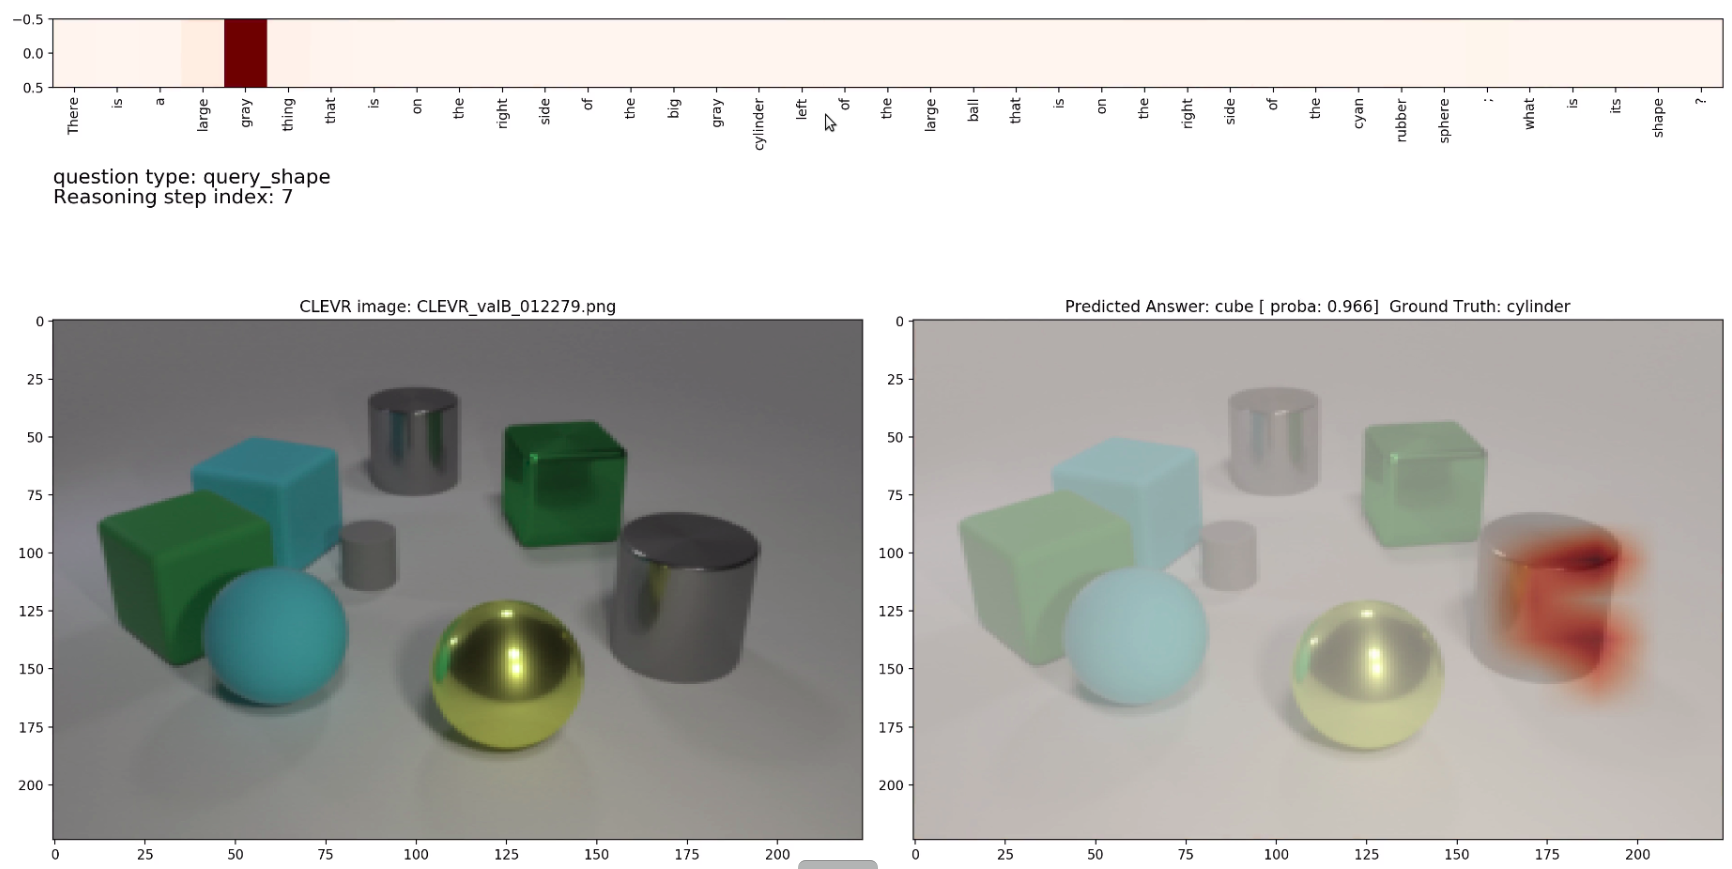
\includegraphics[width=\textwidth]{img/fail_mac_cogent_b_shape.png}
	\caption{The question reads as: \textit{There is a large gray thing that is on the right side of the big gray cylinder left of the large ball that is on the right side if the cyan rubber sphere; what is its shape?}}
	\label{fig:fail_mac_shape}
\end{figure}

\begin{figure}[]
	\centering
	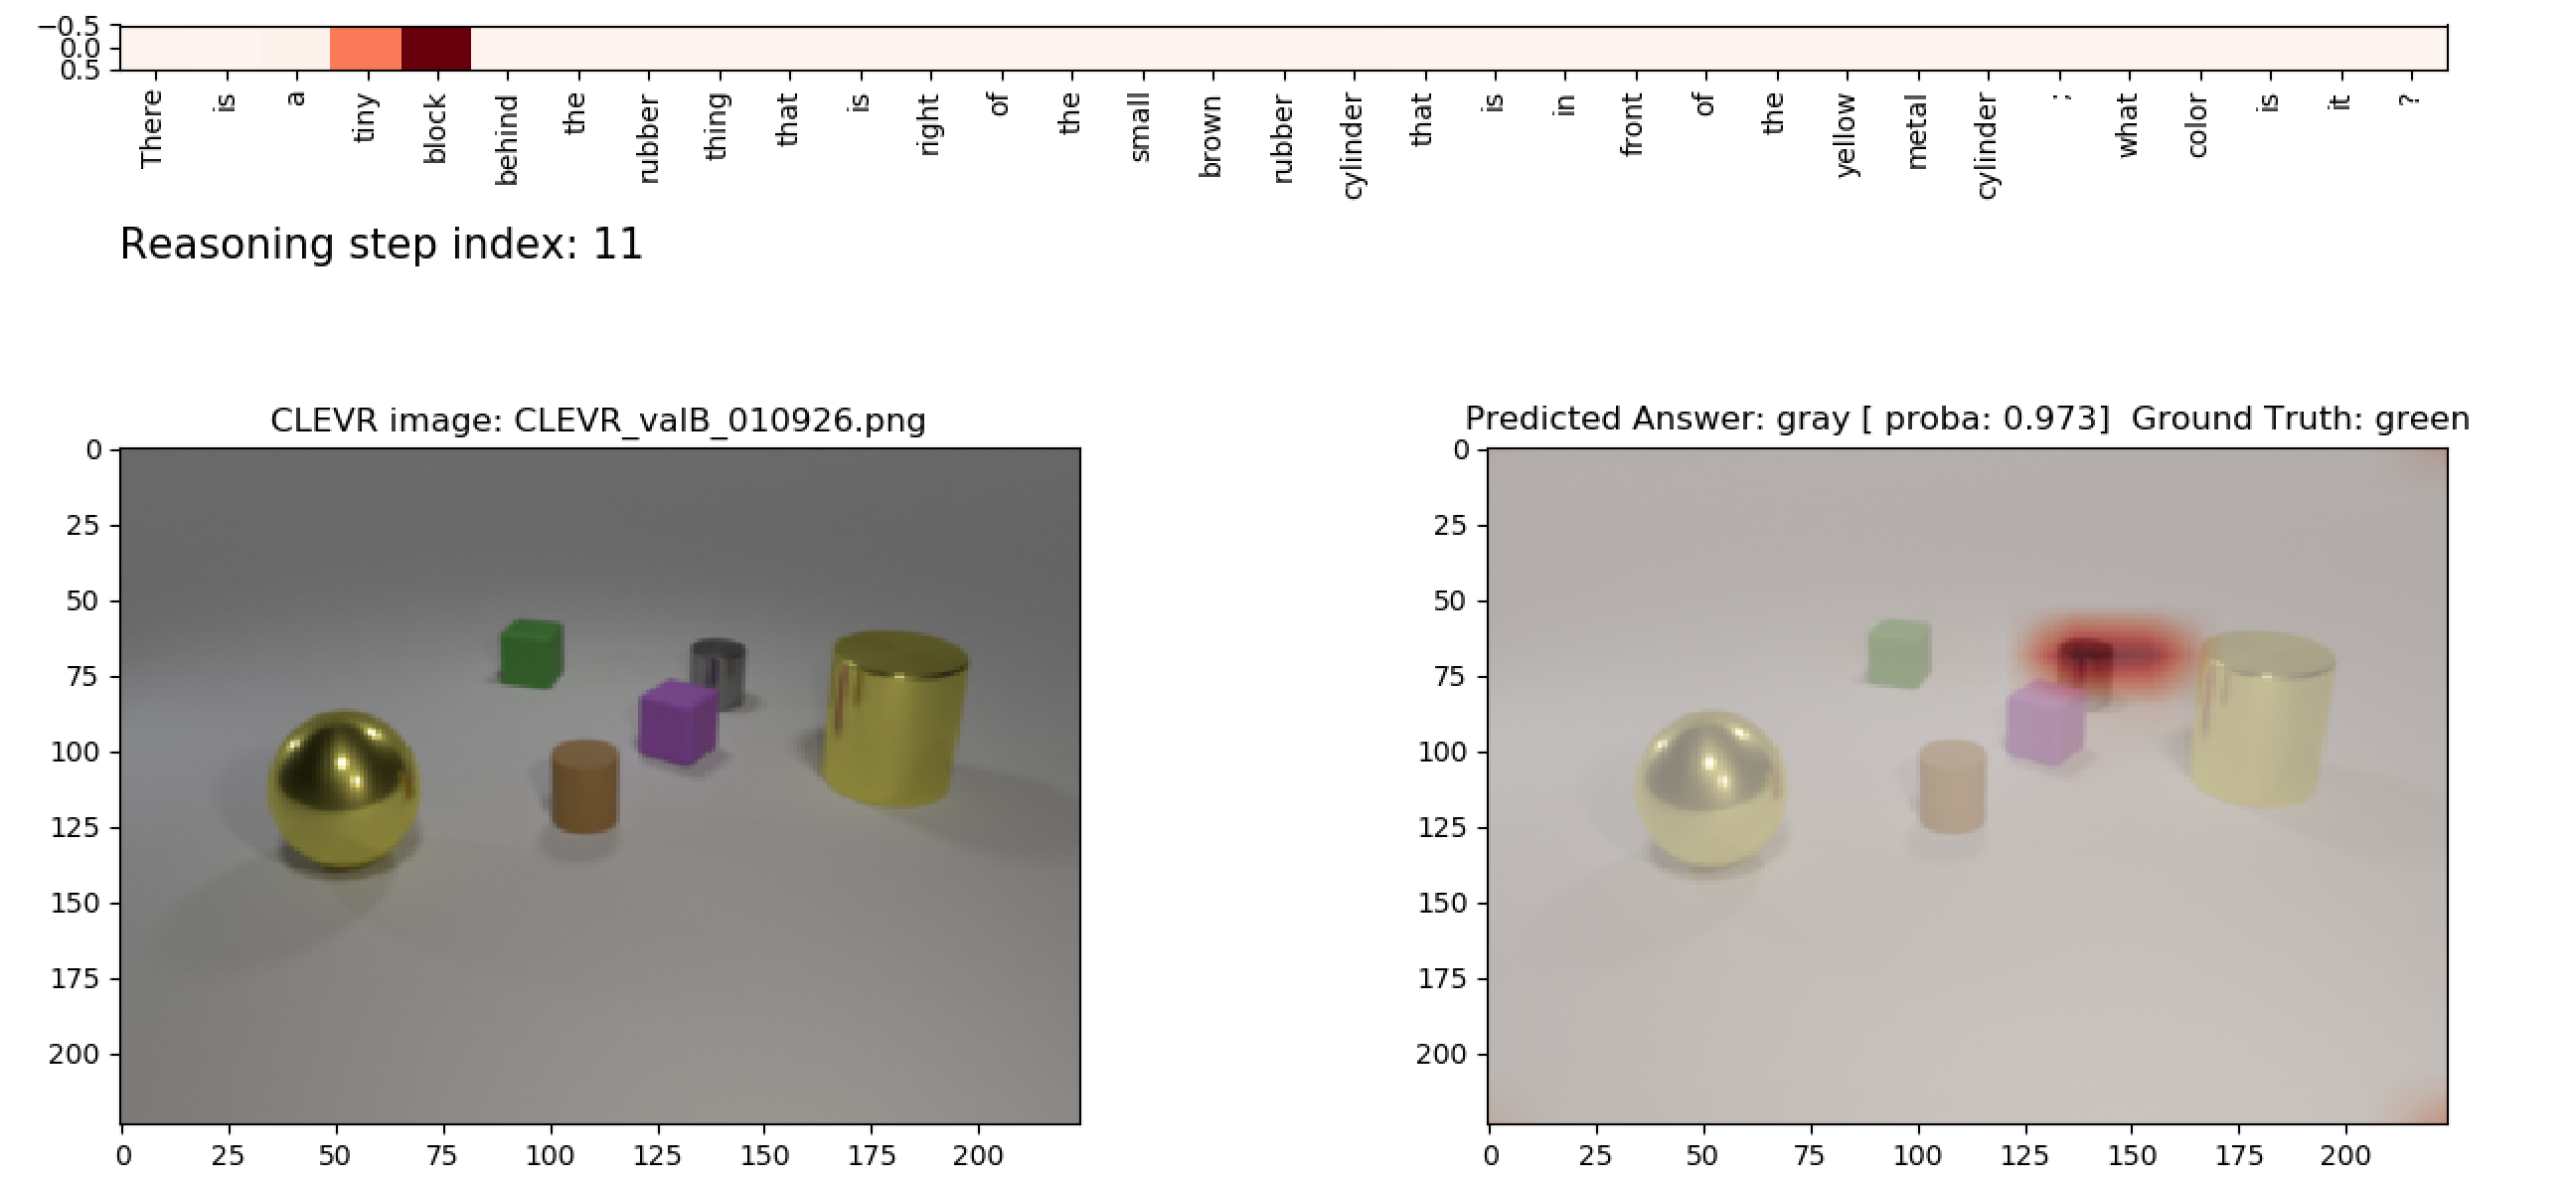
\includegraphics[width=\textwidth]{img/fail_mac_cogent_b_color.png}
	\caption{The question reads as: \textit{There is a tiny block behind the rubber thing that is right if the small brown rubber cylinder that is in front of the yellow metal cylinder; what color is it?}}
	\label{fig:fail_mac_color}
\end{figure}

Those examples indicate that MAC did not correctly separate the concept of shape from the concept of color, but have a better understanding of the colors (as it found the object of interest in \fig{fig:fail_mac_shape} by its color). This could come from that fact that the shape \textit{sphere} is associated with all possible colors in the dataset. 


\newpage
\bibliographystyle{alpha}
\bibliography{../vigil_bibliography}

\end{document}
